\documentclass[letterpaper,12pt]{report} %tipo de documento y tama~o de papel y letra
\usepackage[latin1]{inputenc} %codificacion de caracteres
\usepackage[spanish]{babel} %idioma
\usepackage{fancyhdr} %tipo de pagina, LINDA biggrin.gif
\usepackage[top=3.5cm,bottom=2.5cm,right=2cm,left=2.5cm]{geometry} %margenes
\usepackage[rflt]{floatflt} %ni puta idea
\usepackage{pdfpages} %incluir archivos pdf
\usepackage{hyperref} %hipervinculos
\hypersetup{
  colorlinks=true,
  urlcolor=cyan
}
%\usepackage{helvet} %esto es pa escribir con Arial en vez de times new roman
%\renewcommand\familydefault{\sfdefault} %descomenta estas lineas para escribir en arial

\usepackage{multirow}

\usepackage{graphicx} %para usar imagenes
%\newcommand{\imgdir}{doc-img} % para meter las imagenes en una carpeta especial, tunz en la carpeta del documento tiene q ir otra que se llame 'doc-img'
\graphicspath{{./pic/}} %le dice que las imagenes estan en la carpeta de arriba

\usepackage{amsmath} %pa usar smbolos matematicos
\numberwithin{equation}{section} % pa usar ecuaciones de modo lindo
\numberwithin{figure}{section} %para agregar imagenes
\numberwithin{table}{section} %para agregar tablas

\usepackage{subfigure} % pa usar sub figuras



\pagestyle{fancy} %configuracion para la pagina linda
\renewcommand{\sectionmark}[1]{\markboth{}{\thesection\ \ #1}} %cambios de comentarios
\lhead{} %parte de arriba, izq
\chead{} %parte de arriba, centro
\rhead{\rightmark} %parte de arriba, derecha, le agrega la marca del capitulo
\lfoot{} %parte de abajo, izq
\cfoot{} %parte de abajo, centro
\rfoot{\thepage} %parte de abajo, derecha, va el numero de la pagina


%-------------portada---------------------------------%
\begin{document}
\begin{titlepage} %portada
\thispagestyle{empty} %borrar el formato de pagina linda
%\begin{flushleft} %alinear a la izq
\begin{center}

\includegraphics[scale=0.25]{logoUSM-DI.eps}
%\vfill
\end{center}
%\end{flushleft}

\vspace{3cm} %espacio vertical , en realidad es un enter de 2 cm
\begin{center} %centrar
{\Huge Proyecto ``\emph{V.I.Pe.R.}''\\
 \huge Pre-Empresa {\bf Phyrex} \\
  \normalsize\today
}
\end{center}

\vspace{2cm}
\begin{flushleft}
\begin{table}[h]
    \begin{tabular}{lp{13cm}}
      {\Large \bf Descripci\'on:} & {\large Simulador de mascota que explota caracter\'{\i}sticas de smartphones Android e interact\'ua con robot Lego, enfocado en la difusi\'on del Dpto. de Inform\'atica de la UTFSM.}\\
      & \\
      & \\
      {\Large \bf Problema:} & {\large En las carreras inform\'aticas se encuentre una gran desinformaci\'on respecto a si mismas, adem\'as de una disminuci\'on en la tasa de matr\'{\i}culas anuales, tanto a nivel nacional como mundial, en particular en el caso de la UTFSM.}\\
    \end{tabular}
\end{table}
\end{flushleft}

%\vspace{6cm}
\vfill
\begin{flushleft} %alinear derecha
\begin{table}[hb]
  \begin{tabular}{lllc}
    Jefe de Proyecto: & Rodrigo Fr\'{\i}as & \texttt{\small <rodrigo.frias@alumnos.usm.cl>} & [+56 9 83988257] \\
    Equipo: & Celeste Bertin & \texttt{\small <celeste.bertin@alumnos.usm.cl>} &[+56 9 68410901]\\
    & Patricio Carrasco &\texttt{\small <patricio.carrascod@alumnos.usm.cl>} &[+56 9 50626689]\\
    & Rocio Fernandez &\texttt{\small <rocio.fernandezu@alumnos.usm.cl>} &[+56 9 62426549]\\
    Categor\'{\i}a: & \multicolumn{3}{l}{Educaci\'on \& Entretenimiento.}\\
    Campus: & \multicolumn{3}{l}{Santiago San Joaqu\'{\i}n.}
  \end{tabular}
\end{table}
\end{flushleft}
\end{titlepage}
%------------------fin de la portada --------------------%

%{\bf } %escribir en negrita

\setcounter{page}{1} %empezar enumerando la pagina 1

\tableofcontents indice
\newpage

\chapter*{Propuesta T\'ecnica}
\newpage
\section{Identificaci\'on del problema u oportunidad}
Actualmente en la las carreras de inform\'atica, espec\'{\i}ficamente en la Universidad T\'ecnica Federico Santa Mar\'{\i}a se ha notado una baja en el n\'umero de estudiantes que postulan por a\~no a las carreras de inform\'atica y han bajado los puntajes PSU de dichos postulantes. Adem\'as, un gran porcentaje de alumnos se retiran de la carrera o se cambian a otra carrera dentro de la universidad desde inform\'atica, llegando a una tasa de retenci\'on aproximada del 50 por ciento.\\~\\
El Departamento de Inform\'atica de la Universidad T\'ecnica Federico Santa Mar\'{\i} est\'a interesado en propuestas que ayuden a cambiar esa tendencia a trav\'es de nuevos m\'etodos de difusi\'on a colegios, espec\'{\i}ficamente difusi\'on que muestre la carrera de inform\'atica de formas fuera del estereotipo de que es un inform\'atico y de manera did\'actica.\\~\\
El segmento de clientes seria estudiantes escolares desde al menos s\'eptimo b\'asico. Mientras m\'as j\'ovenes mejor, ya que desde cierta edad los ni\~nos se cierran a estudiar una carrera STEM (Science, Technology, Engineering, Math) por temas culturales, estereotipos negativos y falta de apoyo en casa.\\~\\
Posibles causales de este problema es que cultualmente, no se tiene una buena noci\'on sobre lo que es ser inform\'atico. Se tiene la noci\'on de que un inform\'atico es alguien quien trabajar\'a toda su vida pegado frente a un computador, o que es alguien que simplemente arreglar\'a computadores y utiliza redes sociales todo el d\'{\i}a Por estas nociones erradas, mucho no consideran inform\'atica como una carrera a seguir, o entran a esta carrera con ideas erradas sobre que es la inform\'atica, y terminan retir\'andose al darse cuenta que no es algo en lo cual les interese trabajar a futuro. No ayuda a esta situaci\'on que los medios no muestran mucho sobre TI, o dan ideas irreales sobre la inform\'atica.\\~\\
Los antecedentes cuantitativos avalan lo anterior. Aproximadamente 50 por ciento de los que entran a ingenier\'{\i}a inform\'atica en la T\'ecnica Federico Santa Mar\'{\i}a se retiran. Aunque no hay estudios formales, esto se nota al ver los ramos anuales de la carrera, en que se tienen alrededor de 50 estudiantes, siendo que cada a\~no entran alrededor de 100 alumnos nuevos a inform\'atica. En una actividad de difusi\'on con 34 alumnos de primero medio, en una encuesta efectuada antes del evento, cerca del 50 por ciento dijo no conocer a alguien en que trabaje en TI, la mayor\'{\i}a, al preguntarles de que se trata la inform\'atica respond\'{\i}an con variaciones de ``trabajan con computadores'', mostrando que en general, no saben que hacen los inform\'aticos. Aunque no saben de qu\'e se trata la inform\'atica, un 55 por ciento le parece una opci\'on entretenida de trabajo. Esto puede darse a que la mayor\'{\i}a usa el computador para ver redes sociales como Facebook.\\~\\
A pesar de que a la mayor\'{\i}a le pareci\'o una opci\'on entretenida de trabajo la inform\'atica, solo 10 de los 34 estar\'{\i}an interesados a trabajar en inform\'atica a futuro. En las encuestas efectuadas despu\'es de la actividad de difusi\'on, las actividades m\'as populares entre los asistentes fueron actividad de interfaces con 66,6\% d\'andole nota entre 6 y 7, y la actividad de Scratch (ambiente de lenguaje de programaci\'on para principiantes), la cual recibi\'o nota 7 de un 66,6\% de los asistentes, mientras que otras actividades como videos testimoniales, la cual recibi\'o un 25,9\% de notas 3-4, y mundo TI en Chile, la cual recibi\'o 62,9\% de notas 5-6, fueron menos populares entre los asistentes. Estos datos muestran que una iniciativa de difusi\'on en la cual los asistentes puedan interactuar son las m\'as efectivas. Al finalizar la actividad de difusi\'on, 32\% de los asistentes se declararon m\'as dispuestos a trabajar en inform\'atica en el futuro, comparado con un solo asistente que se declar\'o menos dispuesto a trabajar en inform\'atica a futuro. En general, al terminar el evento, los asistentes ten\'{\i}an una idea m\'as concreta sobre que hace un inform\'atico.

\newpage
\section{Visualizaci\'on de una soluci\'on}
Ante las problem\'aticas expuestas en la secci\'on anterior, aspiramos a entregar una propuesta creativa, factible y que maximice los beneficios al Departamento de Inform\'atica, nuestro cliente. La soluci\'on propuesta es una aplicaci\'on m\'ovil que emule una mascota virtual, la cual interactuar\'a con un sistema de Invenci\'on Robotizado por medio de Bluetooth. Cada vez que se encuentren conectados, existir\'a una correlaci\'on inmediata entre las acciones que se efect\'ue con la mascota, o el tel\'efono con la aplicaci\'on en curso, y las reacciones que tenga la mascota ``robot''. La aplicaci\'on funcionar\'{\i}a como el ``cerebro'' de la estructura f\'{\i}sica, y el robot podr\'{\i}a interactuar tanto con el ambiente como con la aplicaci\'on en s\'{\i}. La tecnolog\'{\i}a que se utilizar\'a corresponde a los smartphones con sistema operativo Android, mientras que la parte rob\'otica la aporta Lego Mindstorms NXT. La uni\'on de estos recursos es una alternativa que permite dar a conocer parte de la amplitud de rubros que abarca las carreras Inform\'aticas que imparte la universidad de manera interactiva y novedosa, dando a conocer una amplia gama de herramientas unificadas, generando apego y participaci\'on en la audiencia principal del cliente.\\~\\
La Propuesta de Valor que nuestro proyecto otorga tiene cierto car\'acter social: apuntar a un conocimiento m\'as profundo y a un mayor grado de  inter\'es en la carrera recurriendo a un proyecto llamativo, motivar a quienes tienen habilidades, o quienes est\'en dispuestos y tengan \'animos de conocer y aprender, para ingresar a una rama que puede ofrecer soluciones integrales en variados \'ambitos del quehacer humano. Adicionalmente, esta idea busca incrementar localmente la cantidad de alumnos que ingresan anualmente, y disminuir la taza de deserci\'on debido a la desinformaci\'on y prejuicios existentes actualmente respecto a esta profesi\'on. Existen eventos paralelos con una comunidad muy activa que impulsan la masificaci\'on de nuestra idea a largo plazo. El ejemplo m\'as reciente es la IV Interescolar de Rob\'otica.\\~\\
Si bien es una opci\'on factible cuyos recursos son de f\'acil acceso,  el kit rob\'otico tiene caracter\'{\i}sticas de hardware bastante limitadas, como el microcontrolador, la memoria, cantidad de entradas para sensores, cantidad de salidas para energ\'{\i}a, entre otros. Esto puede dificultar bastante el nivel de interactividad que pueda existir entre el dispositivo m\'ovil y la ``mascota''. Buscamos un \'optimo uso de las capacidades que ambos aparatos puedan ofrecer. Otro desaf\'{\i}o a superar  es la compatibilidad y enriquecimiento de la aplicaci\'on en dispositivos con diferente versi\'on de Android, con especial \'enfasis en aquellos dispositivos de gama media-baja los cuales tambi\'en se encuentran limitados por su capacidad de hardware. Una restricci\'on a considerar que es de importancia es el \'unico medio de comunicaci\'on entre la mascota virtual y la mascota f\'{\i}sica: Bluetooth. Por lo tanto, uno de los punto cr\'{\i}ticos que hay que tener en cuenta en la totalidad del desarrollo del proyecto es mantener la capacidad  de conexi\'on entre ellos por este medio, teniendo en cuenta las propiedades inherentes de esta red inal\'ambrica.\\~\\
Cabe destacar que el Departamento de Inform\'atica facilita una gran parte de los recursos a utilizar, adem\'as tenemos contacto con organizaciones locales relacionadas con la tecnolog\'{\i}a rob\'otica a usar, como la Sociedad Chilena de Ciencia de la Computaci\'on, en busca de apoyo y futura participaci\'on.
\newpage
\section{Innovaci\'on}
Actualmente las tecnolog\'{\i}as tanto virtual como f\'{\i}sicas se han trabajado por separadas en el dise\~no de mascotas virtuales, lo que se ve reflejado en sistemas de simulaci\'on que no logran ser completamente realistas ni lo suficientemente interactivos.\\~\\
Las mascotas rob\'oticas a pesar de tener un medio f\'{\i}sico, no presentan simulaci\'on muy completa de necesidades vitales de un ser vivo tales como dormir, higiene o crecimiento  del animal, esto debido a que se ven limitados por el hardware en si, por lo que se limita a alimentarlos por medio de objetos o sensores espec\'{\i}ficos, jugar o  interactuar entre ellos , lo que finalmente genera una mascota f\'{\i}sica que se limita a jugar pero no tiene necesidades reales.\\~\\
Las mascotas virtuales, a diferencia de las rob\'oticas no tienen una forma f\'{\i}sica concreta aparte del hardware donde se ejecutan. La interacci\'on con las mascotas virtuales puede tener o no objetivo. En el primer caso, el usuario puede tener que mantenerlo vivo tanto como le sea posible , a menudo ayudarlos a crecer. Mantener viva la mascota a menudo exige alimentarla, limpiarla y jugar con ella. Cuando la mascota no tiene un real objetivo se convierte en un juego para el usuario.  A menudo estos sistemas usan efectos visuales o interacciones realistas para hacer que la mascota parezca viva y d\'e sensaci\'on de realismo a los usuarios, aunque la tecnolog\'{\i}a de las mascotas virtuales a avanzado con los a\~nos, y cada vez se intenta recrear de manera m\'as realista la interacci\'on entre el usuario y la mascota , utilizando micr\'ofono, c\'amaras, pantallas t\'actiles u otros elementos  para simular su cuidado, lo que no es suficiente para generar una sensaci\'on de realismo. \\~\\
Se intentara unificar  ambas tecnolog\'{\i}as, tanto la  digital y como la rob\'otica para obtener una simulaci\'on de mascota mas real y cercana a la persona, para esto se utilizara un Smartphone android que utilizar\'a diversos  sensores y caracter\'{\i}sticas del tel\'efono para simular una mascota digital la cual mediante la utilizaci\'on de Bluetooth estar\'a conectada  con un robot de Lego Mindstorms dando la impresi\'on de ser uno solo.\\~\\
Debido a que la intenci\'on de este proyecto  es difundir  el ingreso a ingeniera civil inform\'atica, se detectan dos posibles competidores en el mercado nacional, estos son:\\~\\
La escuela de verano de la Universidad de Chile que a partir de enero del presente a\~no comenz\'o a impartir  un curso de rob\'otica, dise\~no, construcci\'on y programaci\'on, para alumnos de 8° b\'asico, en el cual se intenta acercar a los alumnos a las ciencias F\'{\i}sicas y matem\'aticas mediante el uso y programaci\'on de robos Lego Mindstorms.\\~\\
Tambi\'en existe el "Interescolar de Rob\'otica", el cual ya va en su cuarta versi\'on,  y es un evento que se inici\'o el  a\~no 2010 bajo el alero del Centro de Rob\'otica de la Universidad T\'ecnica Federico Santa Mar\'{\i}a como parte del proyecto "Introducci\'on a la Rob\'otica para Escolares". Su finalidad es acercar a los escolares al \'area de la rob\'otica como tambi\'en desarrollar su ingenio y trabajo en equipo, a trav\'es de distintos desaf\'{\i}os que se relacionan con problemas de contingencia actual.\\~\\
Sin embargo, existen muchos productos relacionados con la simulaci\'on de mascotas, ya sean f\'{\i}sicos como virtuales,  las cuales se venden como juguetes  en su mayor\'{\i}a,  existen en distintas plataformas , por ejemplo:  \\

\begin{itemize}
\item Pou es una aplicaci\'on muy popular para android que simula una mascota con la cual se puede interactuar y jugar. 
\item Tamagotchi es un dispositivo port\'atil el cual simula una mascota la cual se debe criar y cuidar, adem\'as puede interactuar con mascotas de otros dispositivos.  
\item Pet Society es una conocida aplicaci\'on de facebook que la cual cuidas y juegas con una mascota, ademas de compartir con las mascotas de tus contactos. 
\item Petz es una saga de juegos para consolas Nintendo en la cual te encargas de cuidar  perros y gatos, los cuales para el caso de las consolas port\'atiles pueden interactuar con otros.
\end{itemize}
Tambi\'en existen los Simuladores f\'{\i}sicos de mascotas tales como:\\
\begin{itemize}
\item Los Furby que fueron famosos en los a\~nos 2000, los cuales podr\'{\i}as alimentar e interactuaban con otros de su misma clase. 
\item For real friends son mascotas rob\'oticas dise\~nadas para ni\~nas las cuales reaccionan a caricias y realizan gestor similares a las de una mascota real. 
\item Aibo es un robot mascota fabricado por Sony. Tiene forma de perro. Dispone de sensores que le evitan chocar contra objetos,  una cola que funciona de antena, adem\'as de "sentido del tacto" y un simulador de inteligencia artificial.
\end{itemize}
Lo que diferenciar\'{\i}a nuestra idea con otras iniciativas es el enfoque que realizamos, el cual esta dirigido a entretener y captar la atenci\'on de potenciales estudiantes para la universidad,  incorporando el uso de tecnolog\'{\i}as mas cercanas a la gente como lo son los Smatphones. Diferenciando nuestro productos de otros ya existentes, esto al incorporar  la interacci\'on entre medios digitales y fisicos.

\newpage
\chapter*{Anexo I - Presentaci\'on} %Copia Presentacion
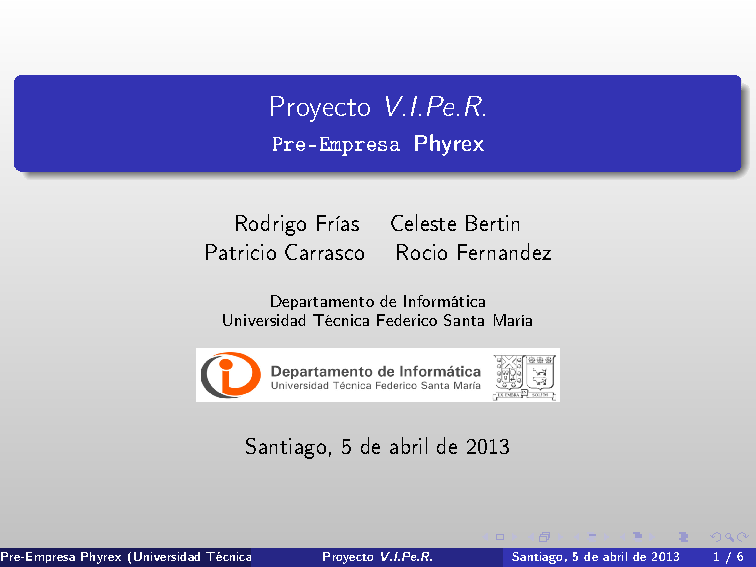
\includepdf[pages={1-},frame=true,nup=2x3,delta=10 20,scale=0.85]{../Presentacion/diapo-1x1.pdf}
\newpage
\chapter*{Anexo II - Curr\'{\i}culum Vitae} %Curriculum
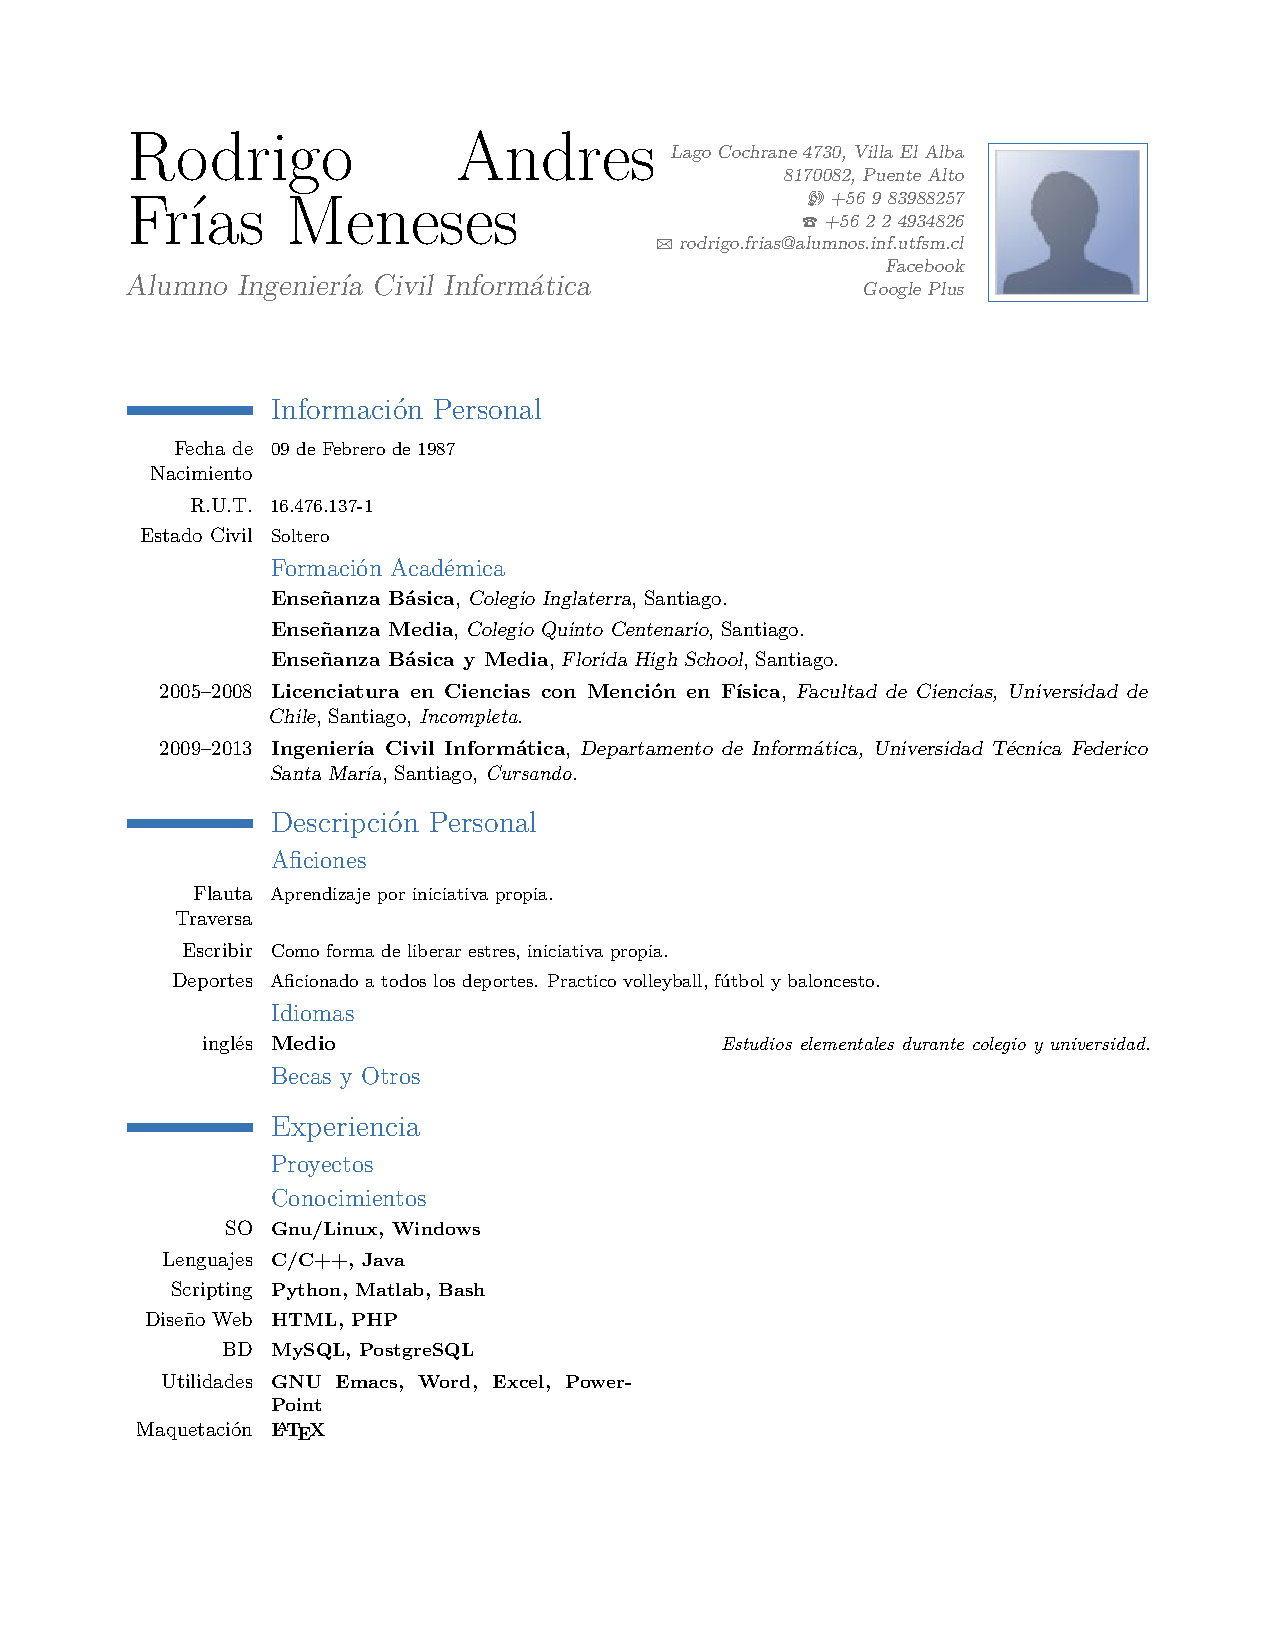
\includepdf[pages={1}]{../CV/cv-igo.pdf}
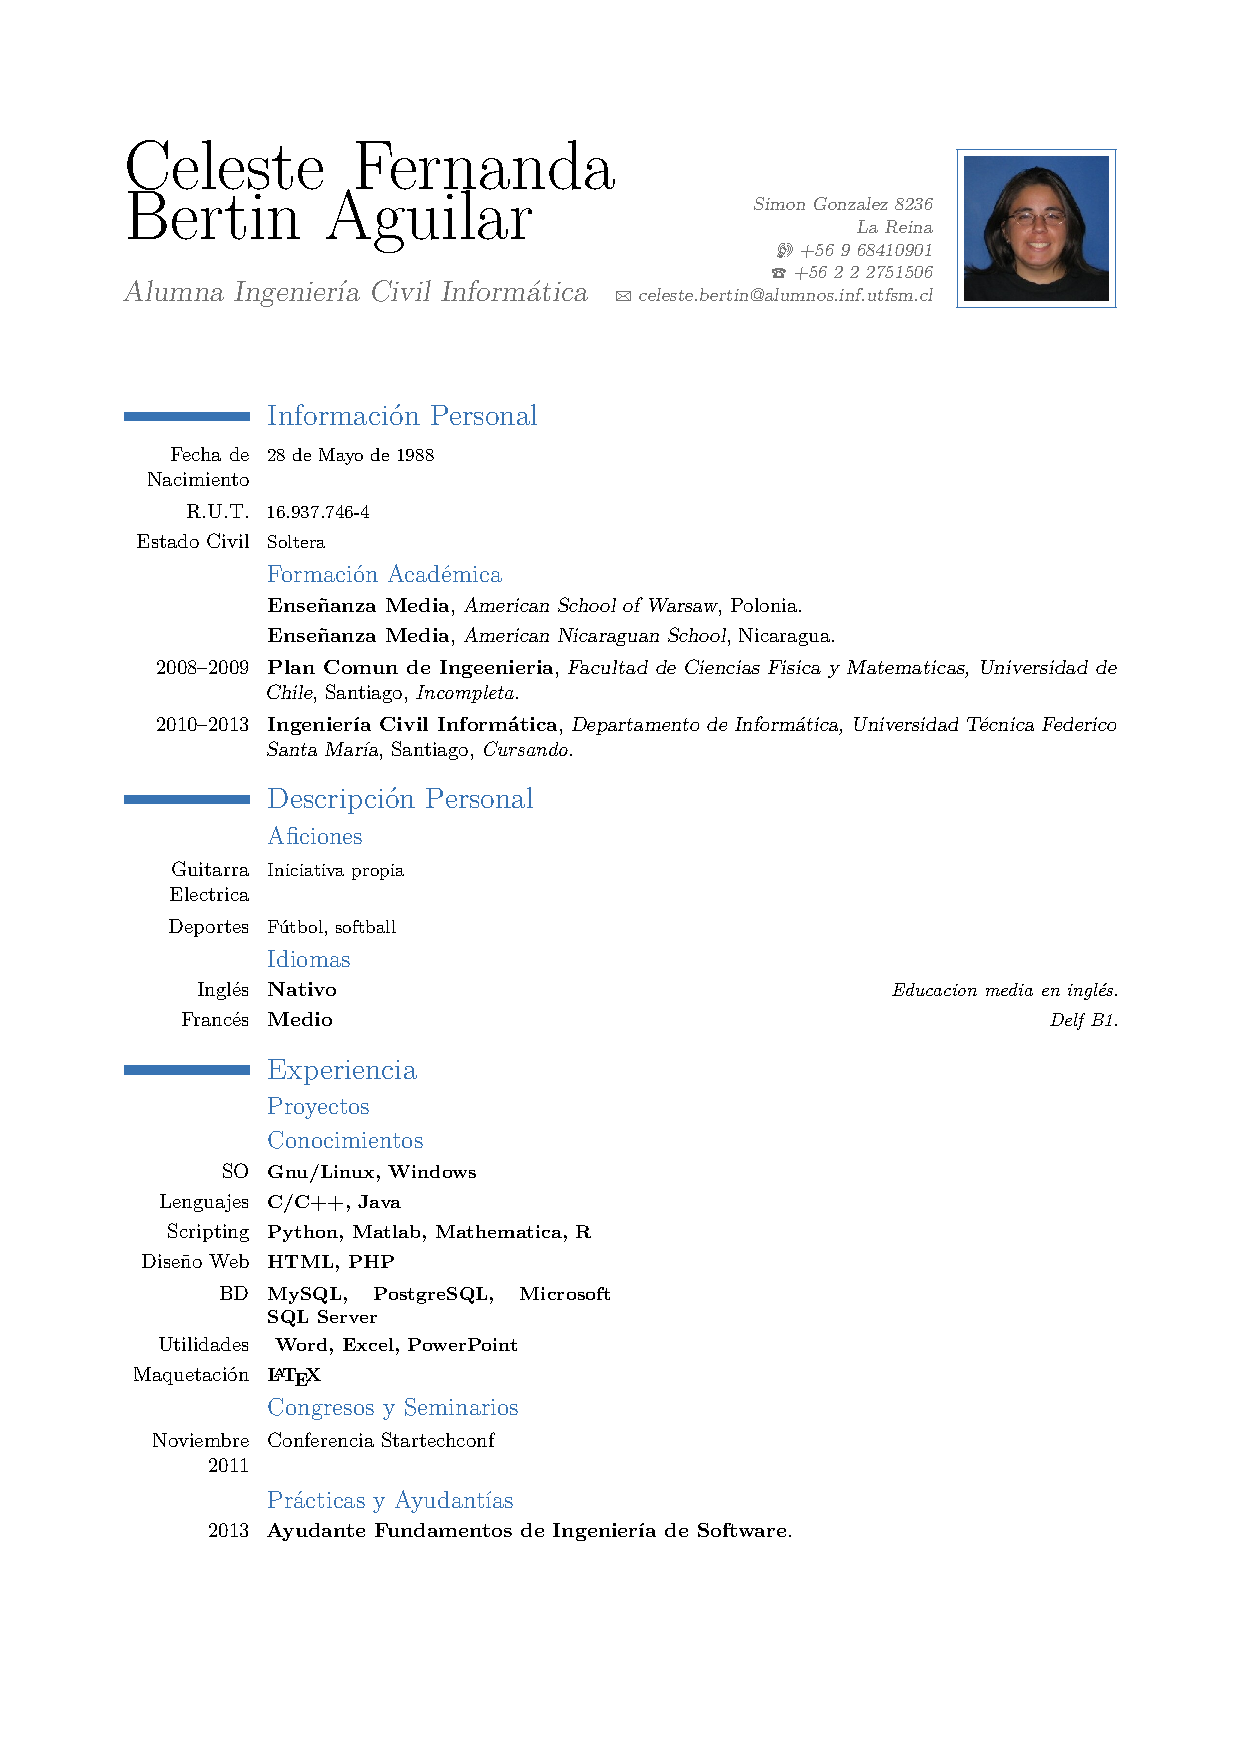
\includepdf[pages={1}]{../CV/cv-celeste.pdf}
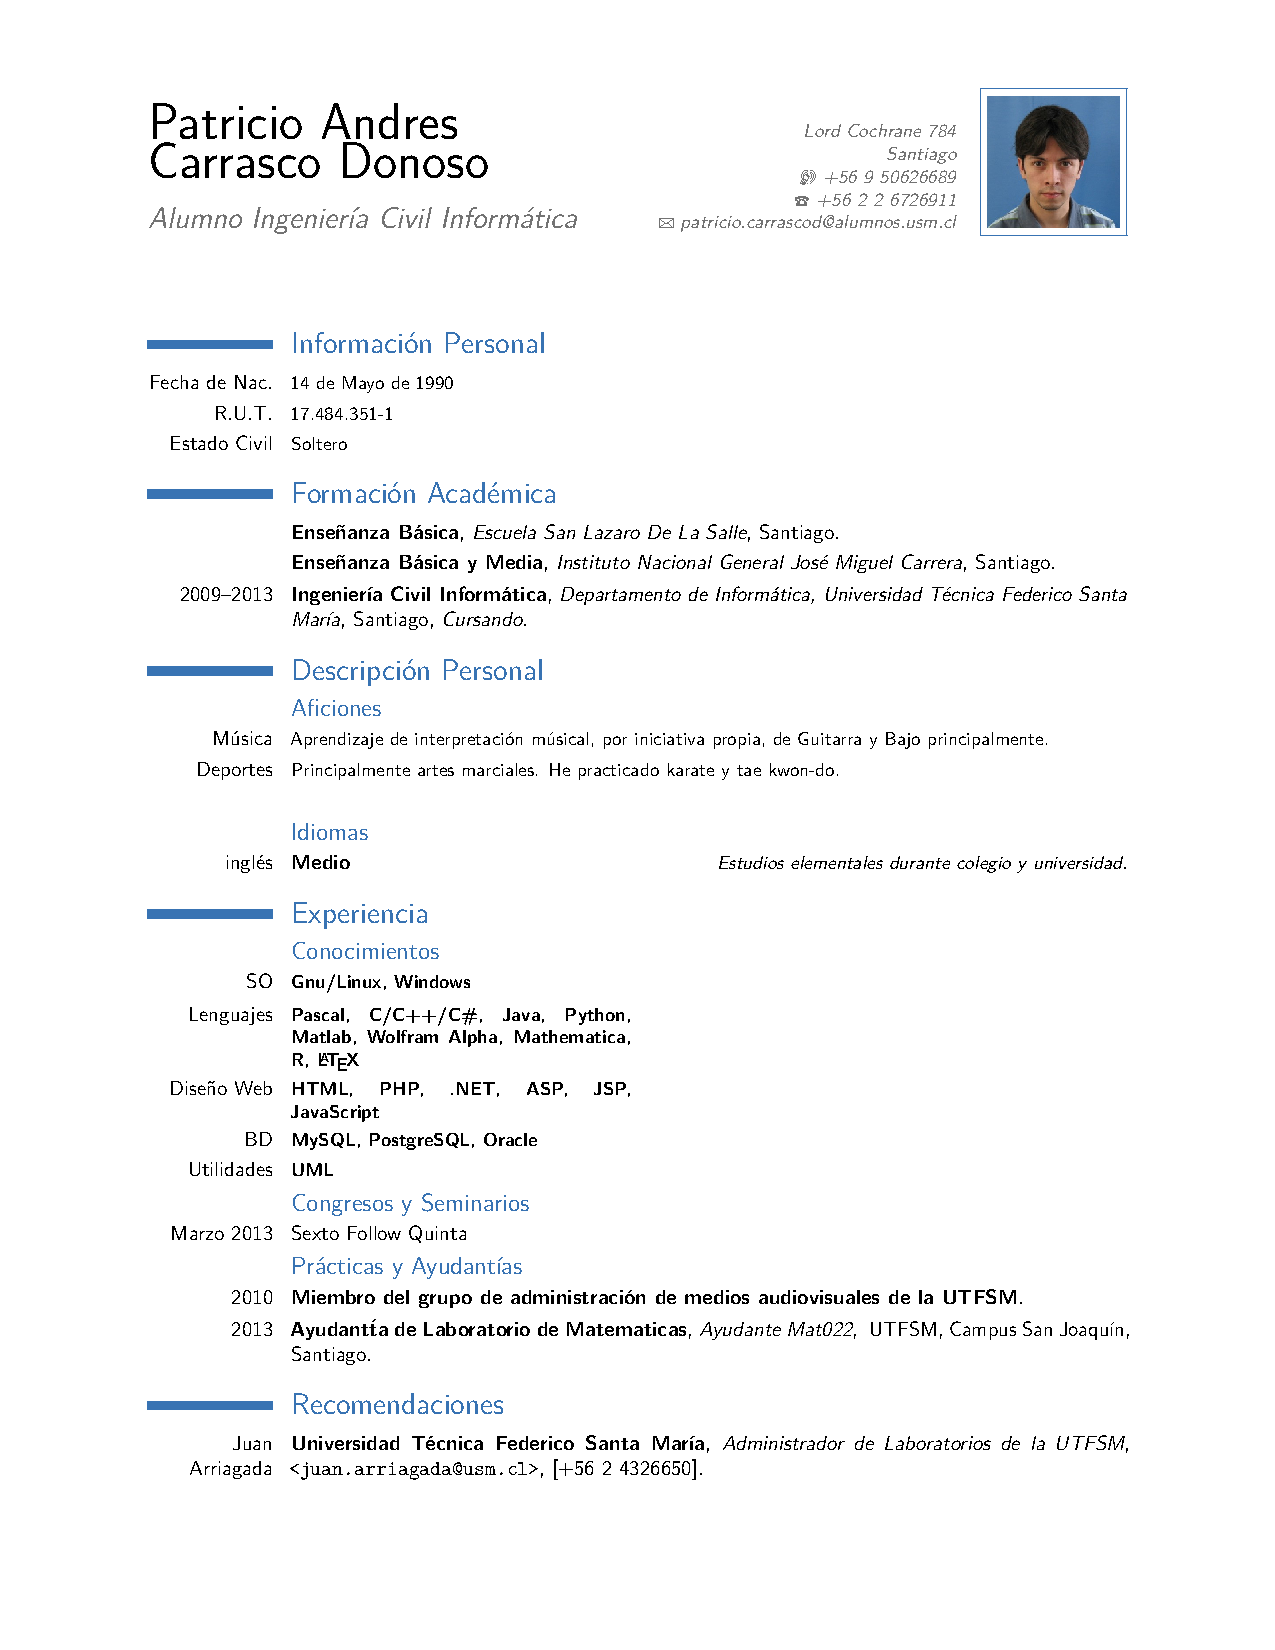
\includepdf[pages={1}]{../CV/cv-pato.pdf}
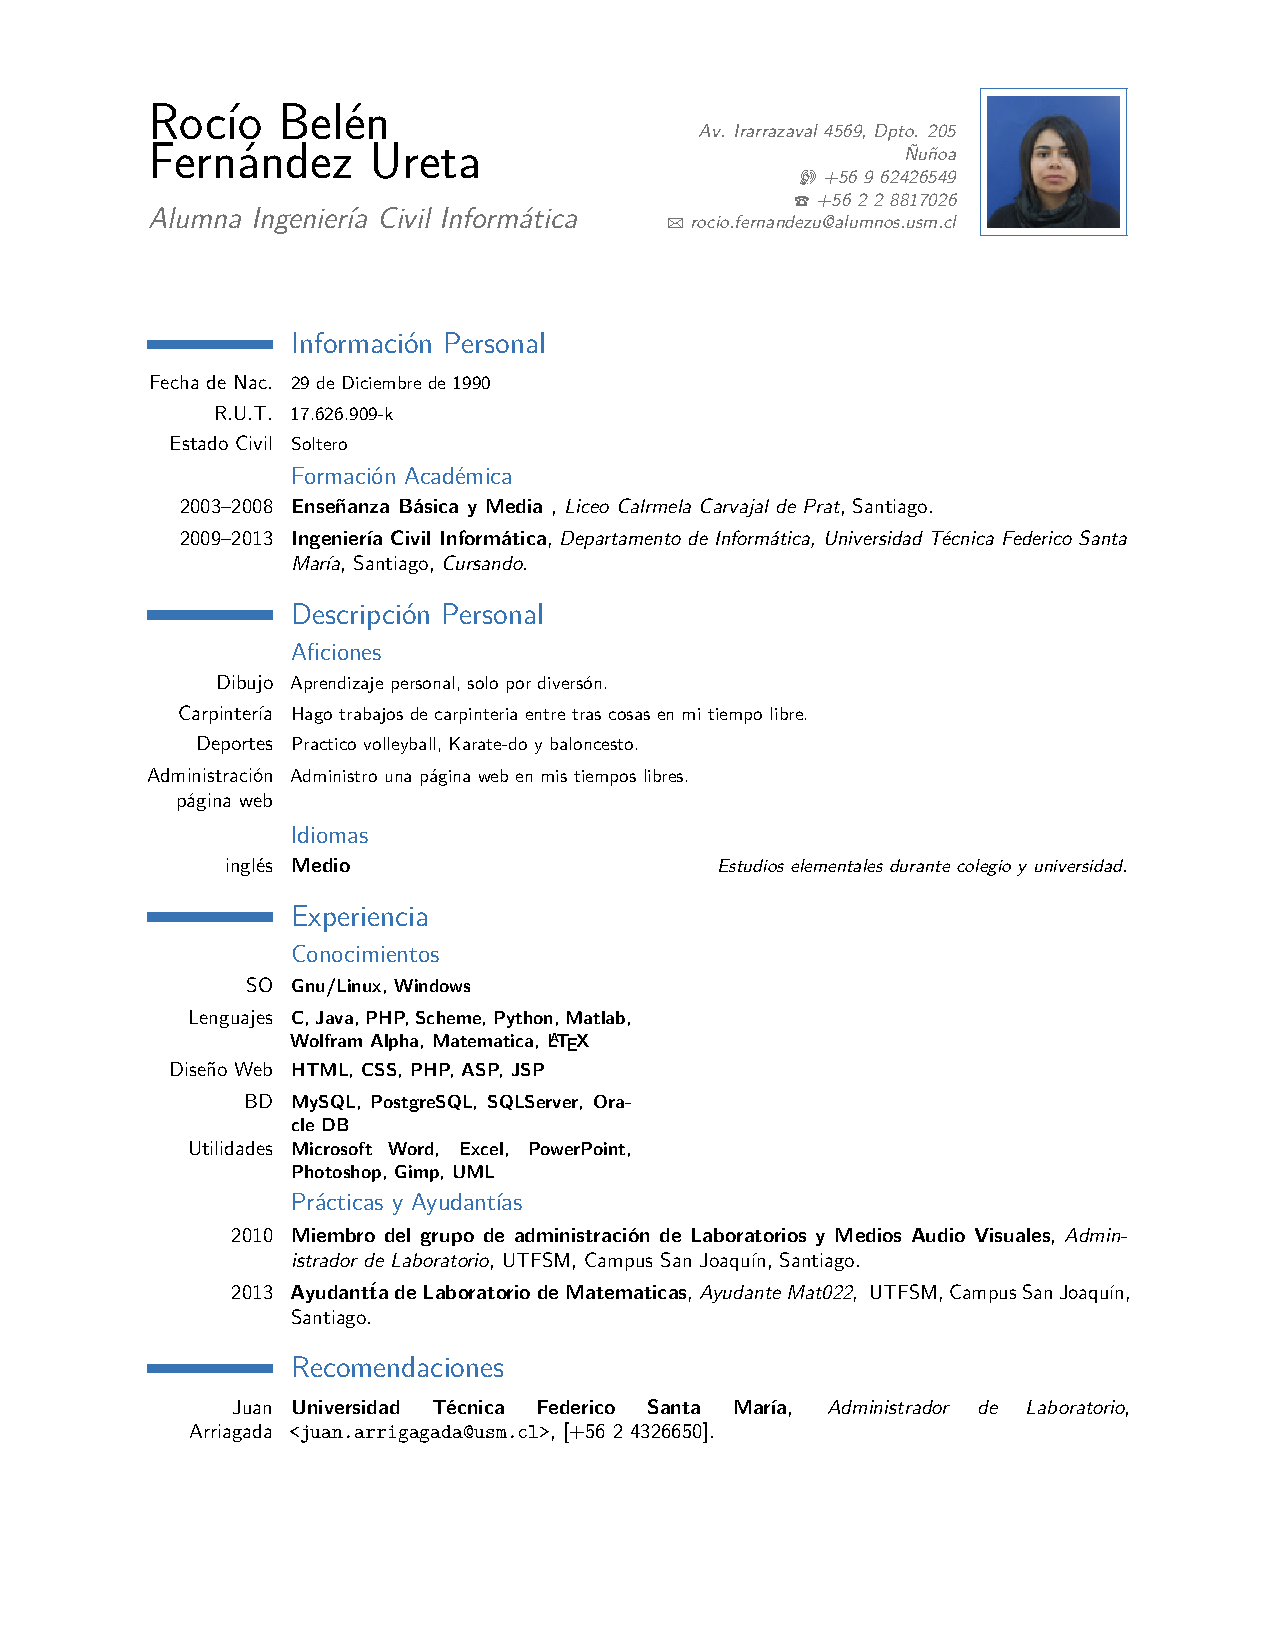
\includepdf[pages={1}]{../CV/cv-neko.pdf}
%\newpage
%\chapter*{Anexo III - Otros} %Otros


\end{document}
